\documentclass[11pt, oneside]{article}   	% use "amsart" instead of "article" for AMSLaTeX format
\usepackage{geometry}                		% See geometry.pdf to learn the layout options. There are lots.
\geometry{letterpaper}                   		% ... or a4paper or a5paper or ... 
%\geometry{landscape}                		% Activate for rotated page geometry
%\usepackage[parfill]{parskip}    		% Activate to begin paragraphs with an empty line rather than an indent
\usepackage{graphicx}				% Use pdf, png, jpg, or eps§ with pdflatex; use eps in DVI mode
								% TeX will automatically convert eps --> pdf in pdflatex		          
\usepackage{amssymb}
\usepackage{amsmath}
\usepackage{xcolor}
\usepackage[normalem]{ulem}
\usepackage{float}
%SetFonts

\usepackage{hyperref} % Required for adding links	and customizing them
\hypersetup{ breaklinks} % Set link colors
\hypersetup{
    colorlinks=true,
    linkcolor=blue,
    filecolor=magenta,      
    urlcolor=cyan,
}

   \def\ci{\perp\!\!\!\perp}

\newcommand{\sophie}[1]{{\color{blue}#1}}
\newcommand{\pablo}[1]{{\color{red}#1}}

\title{HLP Blog post}
\author{The Author}
%\date{}							% Activate to display a given date or no date

\begin{document}
\maketitle

{In the final instalment of the \href{http://www.appliedcategorytheory.org/school/}{Applied Category Theory seminar}, we discussed the 2014 paper  \href{http://iopscience.iop.org/article/10.1088/1367-2630/16/11/113043/meta}{\emph{``Theory-independent limits on correlations from generalized Bayesian networks''}} by Henson, Lal and Pusey. 

In this post, we'll give a short introduction to Bayesian networks, explain why quantum mechanics means that one may want to generalise them, and present the main results of the paper. That's a lot to cover, and there won't be a huge amount of category theory, but we hope to give the reader some intuition about the issues involved, and \href{https://golem.ph.utexas.edu/category/2018/01/a_categorical_semantics_for_ca.html#more}{another} example of monoidal categories used in causal theory.}

\section{Introduction}


Bayesian networks are a graphical modelling tool used to show how random variables interact. A Bayesian network consists of a pair $(G,P)$ of directed acyclic graph (DAG) $G$ together with a joint probability distribution $P$ on its nodes, satisfying the \hyperlink{Markov}{\emph{Markov condition}}. Intuitively the graph describes a flow of information. 

The Markov condition says that the system doesn't have \emph{memory}. That is, the distribution on a given node $Y$ is only dependent on the distributions on the nodes $X$ for which there is an edge $X \rightarrow Y$.
Consider the following chain of binary events. In spring, the pollen in the air may cause someone to have an allergic reaction that may make them sneeze.

{ \begin{figure}[H]
\centering 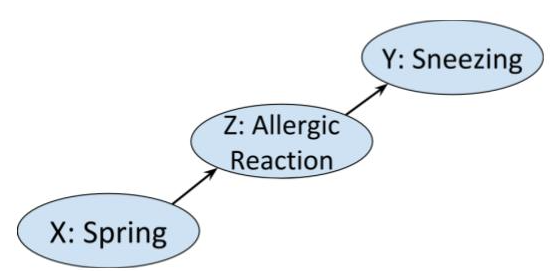
\includegraphics[width= 8cm]{blogpost_figures/fig1.png} \end{figure} }

In this case the Markov condition says that given that you know that someone is having an allergic reaction, whether or not it is spring is not going to influence your belief about the likelihood of them sneezing. Which seems sensible.
\vskip 2ex
Bayesian networks are useful
\begin{itemize}
\item as an inference tool, thanks to \href{https://arxiv.org/abs/1201.4724}{belief propagation} algorithms,
\item and because, given a Bayesian network $(G,P)$, we can describe \hyperref[dsep]{\emph{d-separation}} properties on $G$ which enable us to discover conditional independences in $P$. 

\end{itemize}

It is this second point that we'll be interested in here.
\vskip 2ex


Before getting into the details of the paper, let's try to motivate this discussion by explaining its title: \emph{``Theory-independent limits on correlations from generalized Bayesian networks"} and giving a little more background to the problem it aims to solve. 

Crudely put, the paper aims to generalise a method that assumes \emph{classical mechanics} to one that holds in \emph{quantum} and more general theories. 

Classical mechanics rests on two intuitively reasonable and desirable assumptions, together called \emph{local causality},
\begin{itemize}
\item \textbf{Causality:} Causality is usually treated as a physical primitive. Simply put it is the principle that there is a [partial] ordering of events in space time. In order to have information flow from event \(A\) to event \(B\), \(A\) \textit{must} be in the past of \(B\).

Physicists often define causality in terms of a \emph{discarding} principle: If we ignore the outcome of a physical process, it doesn't matter what process has occurred. Or, put another way, the outcome of a physical process doesn't change the initial conditions. 

\item \textbf{Locality:} {Locality is the assumption that, at any given instant, the values of any particle's properties are independent of any other particle. Intuitively, it says that particles are individual entities that can be understood in isolation of any other particle. 

Physicists usually picture particles as having a private list of \textit{numbers} determining their properties. The principle of locality would be violated if any of the entries of such a list were \textit{a function} whose domain is another particle's property values.}

\end{itemize}

In 1935 \href{https://journals.aps.org/pr/pdf/10.1103/PhysRev.47.777}{Einstein, Podolski and Rosen} showed that quantum mechanics (which was a recently born theory) predicted that a pair of particles could be prepared so that applying an action on one of them would instantaneously affect the other, no matter how distant in space they were, thus contradicting local causality. This seemed so unreasonable that the authors presented it as evidence that quantum mechanics was wrong.

But Einstein was wrong. In 1964, \href{On the Einstein Podolsky Rosen Paradox}{John S. Bell} set the bases for an experimental test that would demonstrate that Einstein's ``spooky action at a distance'' (Einstein's own words), now known as \textit{entanglement}, was indeed real. Bell's experiment has been replicated countless of times and has plenty of variations. \href{https://www.youtube.com/watch?v=MUrXhAxGOWU}{This video} gives a detailed explanation of one of these experiments, for a non-physicist audience.

%\marginpar{\sophie{We could reduce this to the first sentence if necessary, but I like it now.}}

But then, if acting on a particle has an instantaneous effect on a distant point in space, one of the two principle above is violated: On one hand, if we acted on both particles at the same time, each action being a distinct event, both would be affecting each other's result, so it would not be possible to decide on an ordering; causality would be broken. The other option would be to reject locality: {a property's value may be given by \textit{a function}, so the resulting value may \textit{instantaneously} change when the distant `domain' particle is altered. In that case, the particles' information was never separated in space, as they were never truly isolated, so causality is preserved.}

Since causality is integral to our understanding of the world and forms the basis of scientific reasoning, the standard interpretation of quantum mechanics is to accept non-locality.


%\marginpar{\pablo{This is the best I can do to explain non-locality. If you think it's too much text, we may be able to summarise it a bit, know that we have it written down.}}



\vskip 2ex


The definition of Bayesian networks implies a \hyperlink{discard}{discarding principle} and hence there is a formal sense in which they are causal (even if, as we shall see, the correlations they model do not always reflect the temporal order). Under this interpretation, the causal theory Bayesian networks describe is classical. Precisely, they can only model probability distributions that satisfy local causality. Hence, in particular, they are not sufficient to model all physical correlations.



\vskip 2ex

The goal of the paper to develop a framework that generalises Bayesian networks and d-separation results, so that we can still use graph properties to reason about conditional dependence, independently of a given causal theory, be it classical, quantum, or even more general. In particular, this theory will be able to handle all physically observed correlations, and all theoretically postulated correlations.

Though category theory is not mentioned explicitly, the authors achieve their goal by using the categorical framework of \href{https://arxiv.org/pdf/0908.1583.pdf}{\emph{operational probablistic theories} (OPTs)}.


\section{Bayesian networks and d-separation}



Consider the situation in which we have three Boolean random variables. Alice is either \emph{sneezing} or she is not, she either has a  a \emph{fever} or she does not, and she may or may not have \emph{flu}.

Now, flu can cause both sneezing and fever, that is
\[ P(sneezing \ | \ flu ) \neq P( sneezing) \  \text{ and likewise } \ P(fever \ | \ flu ) \neq P( fever) \]
so we could represent this graphically as

{ \begin{figure}[H]
\centering 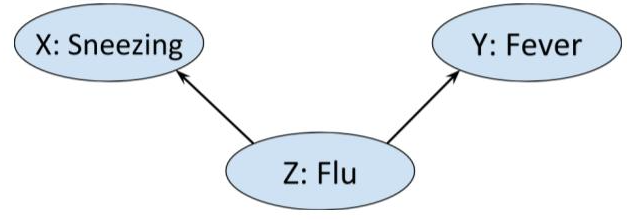
\includegraphics[width= 8cm]{blogpost_figures/fig1b.png} \end{figure} }

Moreover, intuitively we wouldn't expect there to be any other edges in the above graph. Sneezing and fever, though correlated - each is more likely if Alice has flu - are not direct causes of each other.  That is,
\[ P(sneezing \ | \ fever ) \neq P(sneezing) \  \text{ but } \ P(sneezing \ | \ fever, \ flu ) = P(sneezing \ | \ flu).\]




\subsection{Bayesian networks}
Let $G$ be a \emph{directed acyclic graph} or \emph{DAG} $G$. (Here a directed graph is a \href{https://golem.ph.utexas.edu/category/2008/01/mark_weber_on_nerves_of_catego.html}{presheaf on ($ \bullet \rightrightarrows \bullet$)}).

The set $Pa(Y)$ of \emph{parents} of a node $Y$ of $G$ contains those nodes $X$ of $G$ such that there is a directed edge $X \to Y$.

So, in the example above $Pa(flu) = \emptyset$ while $Pa(fever) = Pa(sneezing) = \{ flu \}$.


To each node $X$ of a directed graph $G$, we may associate a random variable, also denoted $X$. If $V$ is the set of nodes of $G$ and $(x_X)_{X \in V}$ is a choice of value $x_X$ for each node $X$, such that $y$ is the chosen value for $Y$, then $pa(y)$ will denote the $Pa(Y)$-tuple of values $(x_X)_{X \in Pa(Y)}$. 


To define Bayesian networks, and establish the notation, let's revise some probability basics.
\\
Let $P(x,y \ | \ z)$ mean $P(X = x \text{ and } \ Y = y \ | \ Z = z)$, the \emph{probability that $X$ has the value $x$, and $Y$ has the value $y$ given that $Z$ has the value $z$}. Recall that this is given by
\[ P(x,y \ |\ z) = \frac{ P(x,y,z) }{P(z)}.\]

The \emph{chain rule} says that, given a value $x$ of $X$ and sets of values $\Omega, \Lambda$ of other random variables, 
\[ P(x, \Omega \ | \ \Lambda) = P( x \ | \ \Lambda) P( \Omega \ | \ x, \Lambda).\]

Random variables $X$ and $Y$ are said to be \emph{conditionally independent given $Z$}, written $X \ci Y \ | \ Z$, if for all values $x$ of $X$, $y$ of $Y$ and $z$ of $Z$
\[ P(x,y \ | \ z) = P(x \ | \ z) P(y \ | \ z).\]

By the chain rule this is equivalent to 
\[ P(x \ | \ y,z )  = P (x \ | \ z) , \ \forall x,y, z. \]

More generally, we may replace $X,Y$ and $Z$ with sets of random variables. So, in the special case that $Z$ is empty, then $X$ and $Y$ are independent if and only if $ P(x, y) = P(x)P(y)$ for all $x,y$.




A joint probability distribution $P$ on the nodes of a DAG $ G$ is said to satisfy the \hypertarget{Markov}{Markov condition} if for any set of random variable $\{X_i\}_{i = 1}^n$ on the nodes of $G$, with choice of values $\{x_i\}_{i = 1}^n$

\[P(x_i, \dots, x_n) = \prod_{i = 1}^n P(x_i \ | \ {pa(x_i)}).\]

So, for the flu, fever and sneezing example above, a distribution $P$ satisfies the Markov condition if
\[ P(flu, \ fever, \ sneezing)  = P(fever \ | \ flu) P(sneezing \ | \ flu) P(flu).\]

A Bayesian network is defined as a pair $(G,P)$ of a DAG $G$ and a joint probability distribution $P$ on the nodes of $G$ that satisfies the Markov condition with respect to $G$. This means that each node in a Bayesian network is conditionally independent, given its parents, of any of the remaining nodes.

In particular, given a Bayesian network $(G,P)$ such that there is a directed edge $X \to Y$, the Markov condition implies that 
\[ \sum_{y} P(x,y) = \sum_y P(x) P(y \ | \ x) = P(x) \sum_y P(y \ | \ x)  = P(x)\] which may be interpreted as a \hypertarget{discard}{discard condition} . (The ordering is reflected by the fact that we can't derive $P(y)$ from $ \sum_{x} P(x,y) = \sum_x P(x) P(y \ | \ x) $.)

%\sout{Crucially, the correlations described by Bayesian networks are classical - they satisfy local causality.} [\pablo{This isn't correct. If you have \(A \to B\) you may have \textit{any} correlation. The whole point is that if you don't want an edge \(A \to B\), because \(A\) and \(B\) may be events that can't possibly signal each other, then you'd like to add a hidden variable \(\Lambda\) forming a fork. The correct claim is that adding a \textit{standard BN node \(\Lambda\) can't explain every possible correlation between A and B.} And that is the reason why we have unobserved nodes. I think this discussion should not be here, but rather in the section about latent/hidden/unobservable variables.]}

 \vskip 2ex
 

Let's consider some simple examples.
\vskip 2ex
\textbf{Fork}\\

In the example of flu, sneezing and fever above, the graph has a \emph{fork} shape. For a probability distribution $P$ to satisfy the Markov condition for this graph we must have
\[ P(x, y, z) = P(x \ | \ z) P(y \ | \ z)P(z), \ \forall x,y,z.\] However, $P(x,y) \neq P(x) P(y)$.

In other words, $X \ci Y   \ | \ Z$, though $X$ and $Y$ are not independent. This makes sense, we wouldn't expect sneezing and fever to be uncorrelated, but given that we know whether or not Alice has flu, telling us that she has fever isn't going to tell us anything about her sneezing.
\vskip 2ex
\textbf{Collider}\\

Reversing the arrows in the fork graph above gives a \emph{collider} as in the following example.

{ \begin{figure}[H]
\centering 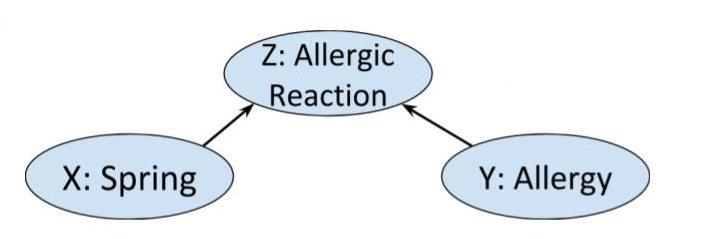
\includegraphics[width= 8cm]{blogpost_figures/fig1c.png} \end{figure} }

Clearly whether or not Alice has allergies other than hayfever is independent of what season it is. So we'd expect a distribution on this graph to satisfy $X \ci Y   \ | \ \emptyset$. However, if we know that Alice is having an allergic reaction, we're going to be far more likely to assume that she has other allergies if we know it's not spring $X$ and $Y$ are not conditionally independent given $Z$.

Indeed, the Markov condition and chain rule for this graph give us
\[ P(x, y, z) = P(x)P(y) P(z \ | \ x,\ y) = P(z \ | \ x,\ y) P( x\ | \ y) P(y) \ \forall x,y,z.\] 
from which we cannot derive $ P(x \ | \ z) P(y \ | \ z) = P(x,y \ | \ z)$. (However, it could still be true, for example if $Z$ is deterministic.)




\vskip 2ex

\textbf{Chain}\\
Finally, let us return the \emph{chain} of correlations presented in the introduction.

Clearly the probabilities that it is spring and that Alice is sneezing are not independent, and indeed, we cannot derive
$P(x, y) = P(x) P(y)$. However observe that, by the chain rule, a Markov distribution on the chain graph must satisfy $X\ci Y   \ | \ Z$. If we know Alice is having an allergic reaction that is not hayfever, whether or not she is sneezing is not going to affect our guess as to what season it is.

Crucially, in this case, knowing the season is also not going to affect whether we think Alice is sneezing. By definition, conditional independence of $X$ and $Y$ given $Z$ is symmetric in $X$ and $Y$. In other words, a joint distribution $P$ on the variables $X,Y,Z$ satisfies the Markov condition with respect to the chain graph 
\[ X \longrightarrow Z \longrightarrow Y \]  if and only if $P$ satisfies the Markov condition on 
\[ Y \longrightarrow  Z \longrightarrow X .\]


\subsection{d-separation}\label{dsep}

The above observations can be generalised to statements about conditional independences in any Bayesian network. That is, if $(G,P)$ is a Bayesian network then the structure of $G$ is enough to derive all the conditional independences in $P$ that are implied by the graph $G$ (in reality there may be more that have not been included in the network!).

Given a DAG $G$ and a set of vertices $U$ of $G$, let $m(U)$ denote the union of $U$ with all the vertices $v$ of $G$ such that there is a directed edge from $U$ to $v$. The set $W(U)$ will denote the \emph{non-inclusive future} of $U$, that is, the set of vertices $v$ of $G$ for which there is no directed (possibly trivial) path from $v$ to $U$. 

For a graph $G$,  let $X, Y, Z$ now be denote disjoint subsets of the vertices of $G$ (and their corresponding random variables). Set $W := W(X \cup Y \cup Z)$.% denote the \emph{non-inclusive future} of $X \cup Y \cup Z$. 

Then $X$ and $Y$ are said to be \emph{d-separated} by $Z$, written $X \perp Y   \ | \ Z$, if there is a partition $\{U,V,W\}$ of the nodes of $ G$ such that 
\begin{itemize}
\item $X \subset U$ and $Y \subset V$, and \item $m(U) \cap m(V) \subset W,$ in other words $U$ and $V$ have no direct influence on each other. \end{itemize} (This is lemma 19 in the paper.)

Now d-separation is really useful since it tells us everything there is to know about the conditional dependences on Bayesian networks with underlying graph $G$. Indeed, 
\vskip 2 ex
THEOREM 5

\begin{itemize} \item \textbf{Soundness of d-separation} (\href{https://www.sciencedirect.com/science/article/pii/B9780444886507500111}{Verma and Pearl, 1988})
If $P$ is a Markov distribution with respect to a graph $G$ then for all disjoint subsets $X,Y,Z$ of nodes of $G$  $X \perp Y   \ | \ Z$ implies that $X,\ci Y   \ | \ Z$.
\item \textbf{Completeness of d-separation} (\href{https://dl.acm.org/citation.cfm?id=2074205}{Meek, 1995})
If $X \ci Y   \ | \ Z$ for all $P$ Markov with respect to $G$, then $ X \perp Y   \ | \ Z$.
\end{itemize}

We can combine the previous examples of fork, collider and chain graphs to get the following

{ \begin{figure}[H]
\centering 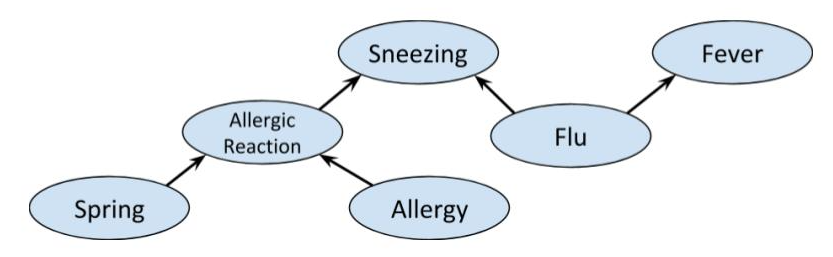
\includegraphics[width= 12cm]{blogpost_figures/fig2.png} \end{figure} }

A priori, \emph{Allergic reaction} is conditionally independent of \emph{Fever}. Indeed, we have the partition

\begin{figure}[H]
\centering 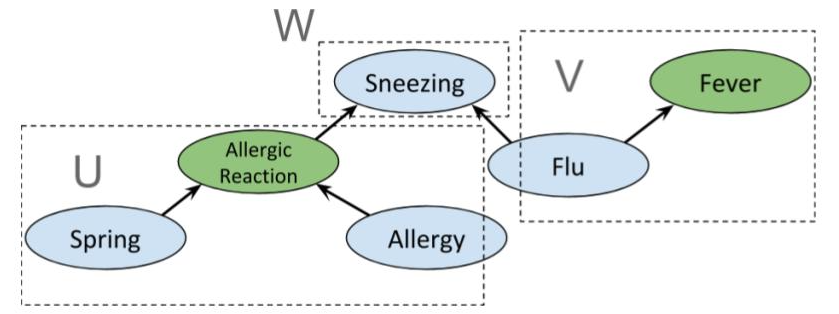
\includegraphics[width= 12cm]{blogpost_figures/fig3.png} \end{figure} 

which clearly satisfies d-separation. However, if \emph{Sneezing} is known, then \emph{Allergic reaction} and \emph{Fever} are not independent. Indeed, in the following partition we have $W = \emptyset$ but $m(U) \cap m(V) = \{ Sneezing \} $.

\begin{figure}[H]
\centering 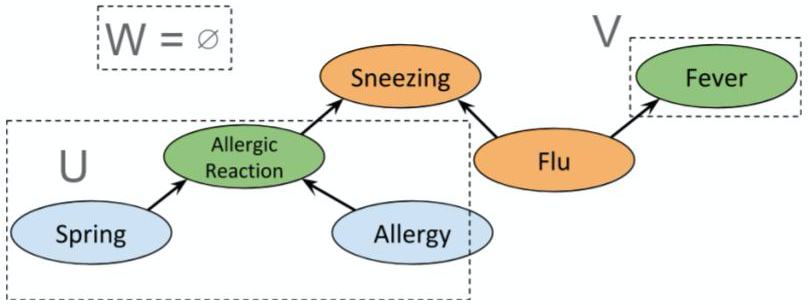
\includegraphics[width= 12cm]{blogpost_figures/fig4.png} \end{figure} 

However, consider what happens what would happen if we added an arrow $Allergy \ \to \ Flu$, then \emph{Allergic Reaction} and \emph{Sneezing} are only conditionally independent if \emph{Allergy} is known. In other cases, we must choose whether to assign \emph{Allergy} to $U$ or $V$, but each option violates d-separation.

\vskip 2ex

Before describing the limitations of this setup and why we may want to generalise it, it is worth observing that Theorem 5 is genuinely useful computationally. Theorem 5 says that given a Bayesian network $(G,P)$, the structure of $G$ gives us a recipe to factor $P$, thereby greatly increasing computation efficiency for Bayesian inference.



\subsection{Latent variables, hidden variables, and unobservables}

In the context of Bayesian networks, there are two reasons that we may wish to add variables to a probabilistic model, even if we are not entirely sure what the variables signify or how they are distributed. The first reason is statistical and the second is physical.

Consider the example of flu, fever and sneezing discussed earlier. Clearly, 
\[ P(fever \ | \ sneezing, \ flu) \neq P(fever \ |  \ flu).\]
%After all, lots of things could cause both sneezing and flu and it's unlikely that we could ever manage to list them all and add them all separately to our network.
%
%In these cases, we may also add hypothetical \emph{latent} variables, just to make the observed distribution Markov. 
%
%In the example,
After all, there are a whole bunch of things that can cause sneezing and flu. We just don't know what they all are or how to measure them.  So, to make the network work, we may add a hypothetical \emph{latent variable} that bunches together all the unknown joint causes, and equip it with a distribution that makes the whole network Bayesian, so that we are still able to perform inference methods like belief propagation.
\begin{figure}[H]
\centering 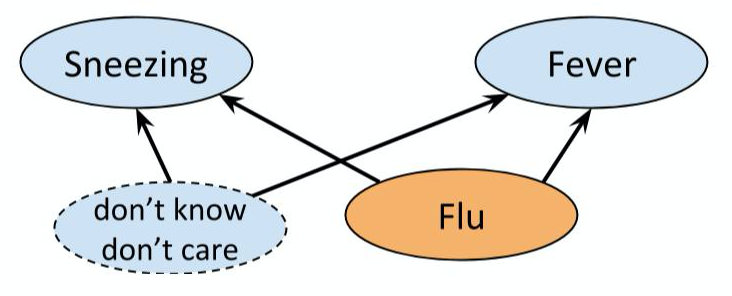
\includegraphics[width= 9cm]{blogpost_figures/fig5.png} \end{figure} 

%There's a saying in computer science that `all models are wrong'.
On the other hand, we may want to add variables to a Bayesian network if we have evidence that doing so will provide a better model of reality. 

For example, consider the network with just two connected nodes
\begin{figure}[H]
\centering 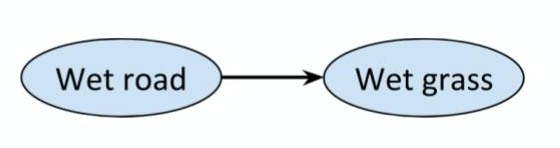
\includegraphics[width= 7cm]{blogpost_figures/fig6.png} \end{figure} 

%\textbf{ Though all cause-effect relationships give correlations, not all correlations are cause-effect.}\\
Every distribution on this graph is Markov, and we would expect there to be a correlation between a road being wet and the grass next to it being wet as well, but most people would claim that there's something missing from the picture. After all, rain could be a `common cause' of the road and the grass being wet. So, it makes sense to add a third variable.  

But maybe we can't observe whether it has rained or not, only whether the grass and/or road are wet. Nonetheless, the correlation we observe suggests that they have a common cause. To deal with such cases, we could make the third variable \emph{hidden}. We may not know what information is included in a hidden variable, nor its probability distribution. 

All that matters is that the hidden variable helps to explain the observed correlations.
 \begin{figure}[H]
\centering 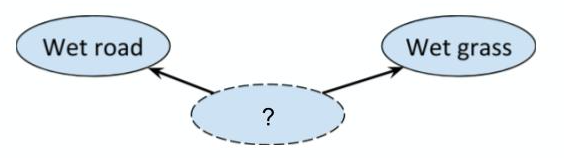
\includegraphics[width= 8cm]{blogpost_figures/fig7.png} \end{figure} 


 
 

So, latent variables are a statistical tool that ensure the Markov condition holds. Hence they are inherently classical, and can, in theory, be known.  But the universe is not classical, so, even if we lump whatever we want into as many classical hidden variables as we want and put them wherever we need, in some cases, there will still be empirically observed correlations that do not satisfy the Markov condition.



Most famously, Bell's experiment shows that it is possible to have distinct variables $A$ and $B$ that exhibit correlations that cannot be explained by any classical hidden variable, since classical variables are restricted by the principle of locality. 

%\sout{In fact, if we define a variable $\Lambda$ as the entire past of $A$ and $B$, so that if we create $A$ and $B$ and make sure nothing else can interact with them, then we know everything about $\Lambda$. Still, we may observe correlations that do not satisfy the Markov condition and are therefore not classically causal.}
%

In other words, though $A \perp B \ | \ \Lambda$, \[ P(a \ | b,\ \lambda) \neq P(a \ | \ \lambda).\]

Implicitly, this means that a \textit{classical} $\Lambda$ is not enough. If we want \(P(a \ | b,\ \lambda) \neq P(a \ | \ \lambda)\) to hold, \(\Lambda\) must be a non-local (non-classical) variable. Quantum mechanics implies that we can't possibly empirically find the value of a non-local variable (for similar reasons to the Heisenberg's uncertainty principle), so non-classical variables are often called \textit{unobservables}. In particular, it is irrelevant to question whether $A \ci B \ | \ \Lambda$, as we would need to know the value of \(\Lambda\) in order to condition over it.

Indeed, this is the key idea behind what follows. We declare certain variables to be unobserved and then insist that conditional (in)
dependence only makes sense between \emph{observable variables conditioned over observable variables}.


%\subsection{Bell's experiment}
%
%LINKS
%
%Alice and Bob each have a particle. They can each measure one of two different properties (for example \emph{position} and \emph{momentum}), and each throws a coin to decide which property to measure.
%
%For some reason, the outcomes of their measurements display correlation.
%\vskip 2ex
%PICTURE SLIDE 19 p 59
%\vskip 2ex
%
%We could assume that the correlation is \emph{caused} by a hidden variable $\Lambda$ that represents the entire past of each particle.
%
%\vskip 2ex
%PICTURE SLIDE 20 p 60
%\vskip 2ex
%
%By theorem 5, $A \ci B \ | \ \Lambda$, so, if we knew $\Lambda$ then $A$ and $B$ would be separated. Moreover, since $\Lambda$ is defined as the entire past of $A$ and $B$, if we create $A$ and $B$ and make sure nothing else can interact with them, then we know everything about $\Lambda$. 
%
%So, there shouldn't be any correlation between $A$ and $B$. However, empirically, there is correlation. That is
%\[ P(a \ | b,\ \lambda) \neq P(a \ | \ \lambda).\]
%
%It seems like Alice and Bob's particle communicate instantaneously with each other across space. The `sensible' solution here is to abandon locality. The state of the pair of particles does not factor into two separate states.
%
%Implicitly, this means that $\Lambda$ is \emph{unobservable}. \emph{We can't know it.} In particular, questions about the validity of $A \ci B \ | \ \Lambda$ are irrelevant.
%
%Indeed, this is the key idea behind what follows. We declare certain variables to be unobservable and then insist that conditional (in) dependence only makes sense between \emph{observable variables conditioned over observable variables}.
%
%
%
%
%%Stronger still, it is not certain that quantum tells the whole story. There are ... (CAN WE GET MAXIMUM CORRELATION? WHAT DOES THIS MEAN WRT d-SEPARATION?)
%



\section{Generalising classical causality}

%\marginpar{ \sophie{Pablo, shall we link to the \href{https://link.springer.com/chapter/10.1007/978-94-017-0990-3_45}{paper} or, e.g. this\href{https://www.scienceandnonduality.com/why-isnt-quantum-mechanics-even-weirder/}{blogpost}? I ask the same question below! \pablo{I would go with a paper in this case, and I prefer this one: https://www.nature.com/articles/nphys2916 (but the one you gave is good too).}}}
The correlations observed in the Bell experiment can be explained by quantum mechanics. But thought experiments such as described  \href{https://www.nature.com/articles/nphys2916}{here} suggest that theoretically, correlations may exist that violate even quantum causality.


So, given that graphical models and d-separation provide such a powerful tool for causal reasoning in the classical context, 
how can we generalise the Markov condition and Theorem 5 to quantum, and even more general causal theories? And, if we have a \emph{theory-independent} Markov condition, are there d-separation results that don't correspond to any given causal theory? 

Clearly the first step in answering these questions is to fix a definition of a \emph{causal} theory.

\subsection{Operational probabalistic theories}

An \href{https://arxiv.org/pdf/0908.1583.pdf}{\emph{operational theory}} is a symmetric monoidal category $(\mathsf C, \otimes, I)$ 
whose objects are known as \emph{systems} or \emph{resources}. Morphisms are finite sets $f = \{\mathcal C_i\}_{i \in I}$ called \emph{tests}, whose elements are called \emph{outcomes}. Tests with a single element are called \emph{deterministic}, and for each system $A \in ob (\mathsf C)$, the identity $id_A \in \mathsf (A,A)$ is a deterministic test.

In this discussion, we'll identify tests $\{\mathcal C_i \}_i , \{\mathcal D_j\}_j$ in $\mathsf C$ if we may always replace one with the other without affecting the distributions in $\mathsf C(I, I)$.


Given $\{\mathcal C_i \}_i \in \mathsf C(B, C)$ and $\{\mathcal D_j \} \in \mathsf C(A, B)$, their composition $f \circ g$ is given by
\[ \{ \mathcal C_i \circ \mathcal D_j \}_{i,j} \in \mathsf C(A, C).\]
First apply $\mathcal D$ with output $B$ then apply $\mathcal C$ with outcome $C$. 

The monoidal composition $\{ \mathcal C_i \otimes \mathcal D_j \}_{i, j} \in \mathsf C(A \otimes C, B \otimes D)$ corresponds to applying $\{\mathcal C_i\}_i \in \mathsf C(A,B)$ and $ \mathcal \{ D_j \}_j$ separately on $ A$ and $C$. 
 
An \emph{operational probabilistic theory} or \emph{OPT} is an operational theory such that every test $I \to I$ is a probability distribution. 

A morphism $\{ \mathcal C_i \}_i \in \mathsf C(A, I)$ is called an \emph{effect} on $A$.  An OPT $\mathsf C$ is called \emph{causal} or a \emph{causal theory} if, for each system $A \in ob (\mathsf C)$, there is a unique deterministic effect $\top_A \in \mathsf C( A, I)$ which we call the \emph{discard} of $A$.

In particular, for a causal OPT $\mathsf C$, uniqueness of the discard implies that, for all systems $A, B \in ob (\mathsf C)$, 
\[ \top_A \otimes \top_B = \top_{A \otimes B},\] and, given any determinstic test $\mathcal C \in \mathsf C(A, B)$,
\[\top_B \circ \mathcal C = \top_A.\]

The existence of a discard map allows a definition of \emph{causal morphisms} in a causal theory. For example, as we saw in \href{https://golem.ph.utexas.edu/category/2018/01/a_categorical_semantics_for_ca.html#more}{January} when we discussed \href{https://arxiv.org/abs/1701.04732}{Kissinger and Uijlen's paper}, a test $\{ \mathcal C_i \}_i \in \mathsf C (A, B)$ is \emph{causal} if 
\[\top_B \circ \{ \mathcal C_i \}_i = \top_A \in \mathsf C( A, I).\]

In other words, for a causal test, discarding the outcome is the same as not performing the test. Intuitively it is not obvious why such morphisms should be called causal. But this definition enables the formulation of a \href{https://golem.ph.utexas.edu/category/2018/01/a_categorical_semantics_for_ca.html#more}{\emph{non-signalling condition}} that describes the conditions under which the possibility of cause-effect correlation is excluded, in particular, it implies the impossibility of time travel.
\vskip 2ex
EXAMPLES\\
The category \href{https://golem.ph.utexas.edu/category/2018/01/a_categorical_semantics_for_ca.html#more}{$Mat(\mathbb R_+)$} of natural numbers and with $Mat(\mathbb R_+)(m,n)$ the set of $n \times m$ matrices, has the structure of a causal OPT.  The causal morphisms in $Mat(\mathbb R_+)$ are the stochastic maps (the matrices whose columns sum to 1). This category describes classical probability theory.

The category \href{https://arxiv.org/abs/1701.04732}{$\mathsf{CPM}$} of sets of linear operators on Hilbert spaces and completely positive maps between them is an OPT and describes quantum relations. The causal morphisms are the trace preserving completely positive maps.

%\marginpar{ \sophie{Pablo, shall we link to the \href{https://link.springer.com/chapter/10.1007/978-94-017-0990-3_45}{paper} or, e.g. this\href{https://www.scienceandnonduality.com/why-isnt-quantum-mechanics-even-weirder/}{blogpost}?}}
Finally, \href{https://www.nature.com/articles/nphys2916}{Boxworld} is the \hypertarget{box}{theory} that allows to describe any correlation between two variables as the cause of some resource of the theory in the past.

\subsection{Generalised Bayesian networks}

So, we're finally ready to give the main construction and results of the paper. As mentioned before, to get a generalised d-separation result, the idea is that we will distinguish observable and unobservable variables, and simply insist that conditional independence is only defined relative to observable variables.

To this end, a \emph{generalised DAG} or \emph{GDAG} is a DAG $G$ together with a partition on the nodes of $G$ into two subsets called \emph{observed} and \emph{unobserved}. We'll represent observed nodes by triangles, and unobserved nodes by circles. An edge out of an (un)observed node will be called \emph{(un)observed} and represented by a (solid) dashed arrow. 

In order to get a generalisation of Theorem 5, we still need to come up with a sensible generalisation of the Markov property which will essential say that at an observed node that has only observed parents, the distribution is Markov. However, if an observed node has an unobserved parent, it's whole history is needed to describe the distribution. 

To state this precisely, we will associate a causal theory $(\mathsf C, \otimes, I)$ to a GDAG $G$  via an assignment of systems to edges of $G$ and tests to nodes of $G$, such that the observed edges of $G$ will `carry' only the outcomes of classical tests (so will say something about conditional probability) whereas unobserved edges will carry only the system output.

Precisely, such an assignment $P$ satisfies the \emph{generalised Markov condition (GMC)} and is called a \emph{generalised Markov distribution} if

\begin{itemize}

\item Each unobserved edge corresponds to a distinct system in the theory.
\item \emph{If we can't observe what is happening at a node, we can't condition over it:}
To each unobserved node and each value of its observed parents, we assign a deterministic test from the system defined by the product of its incoming (unobserved) edges to the system defined by the product of its outgoing (unobserved) edges. 
\item Each observed node $X$ is an observation test, i.e. a morphism in $\mathsf C(A, I)$ for the system $A \in ob( \mathsf C)$ corresponding to the product of the systems assigned to the unobserved input edges of $X$. Since $\mathsf C$ is a causal theory, this says that $X$ is assigned a classical random variable, also denoted $X$, and that if $Y$ is an observed node, and has observed parent $X$, the distribution at $Y$ is conditionally dependent on the distribution at $X$ (see \href{https://arxiv.org/pdf/0908.1583.pdf}{here} for details).\\
It therefore follows that
\item Each observed edge is assigned the trivial system $I$.
\end{itemize}

Note, in particular, that a generalised Markov distribution on a GDAG $G$ defines a joint probability distribution on the nodes of $G$.

A \emph{generalised Bayesian network} consists of a GDAG $G$ together with a generalised Markov distribution $P$ on $G$. \\


EXAMPLE\\
Consider the following GDAG
\begin{figure}[H]
\centering 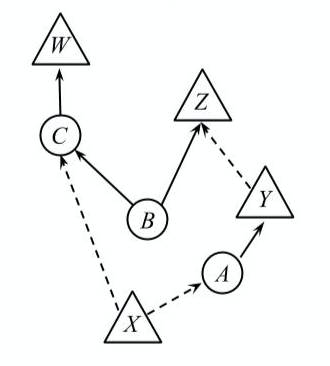
\includegraphics[width= 7cm]{blogpost_figures/fig8.png} \end{figure} 



The observed node $X$ has no incoming edges so we assign a probability distribution.

The unobserved node A \emph{depends} on $X$, and has no unobserved inputs, so we assign a deterministic test $A(x): I \to A$ for each value $x$ of $X$.
\begin{figure}[H]
\centering 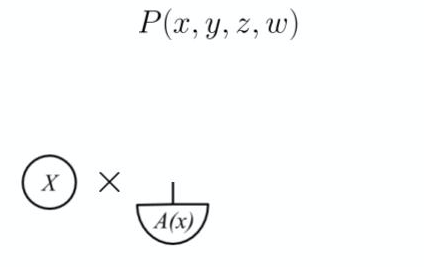
\includegraphics[width= 7cm]{blogpost_figures/fig9.png} \end{figure} 

 The observed node $Y$ has one incoming unobserved edge and no incoming observed edges so we assign to it a test $Y: A \to I$ such that, for each value $x$ of $X$, $Y \circ  A(x)$ is a probability distribution.

Building up the rest of the picture gives an OPT diagram of the form
\begin{figure}[H]
\centering 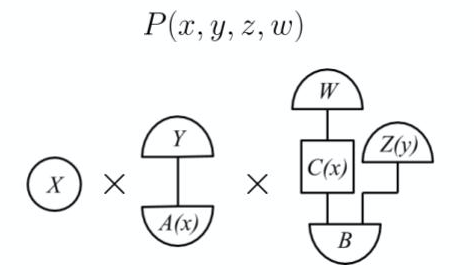
\includegraphics[width= 8cm]{blogpost_figures/fig10.png} \end{figure} 








We now have all the ingredients to state Theorem 22, the \emph{generalised d-separation theorem}. This is the analogue of Theorem 5 for generalised Markov distributions.\vskip 2ex

THEOREM 22

Given a GDAG $G$ and subsets $X,Y, Z$ of observed nodes
\begin{itemize}\item if a probability distribution $P$ is generalised Markov relative to $G$ then $X \perp Y \ | \ Z \Rightarrow  X\ci Y \ | \ Z$.
\item If $ X\ci Y \ | \ Z$ holds for all generalised Markov  probability distributions on $G$, then $X \perp Y \ | \ Z$.
\end{itemize}

Note in particular that there is no change in the definition of d-separation: d-separation of a GDAG $G$ is simply d-separation with respect to its underlying DAG. There is also no change in the definition of conditional independence. Now, however, we restrict to statements of conditional independence with respect to only observed nodes. This enables the generalised soundness and completeness statements of the theorem.


The proof of soundness uses uniqueness of discarding, and completeness follows since generalised Markov is a stronger condition on a distribution than classically Markov.

\subsection{Classical distributions on GDAGs}
Theorem 22 is all well and good. But does it really generalise the classical case? That is, can we recover Theorem 5 for all classical Bayesian networks from Theorem 22?

As a first step, Proposition 17 states that if all the nodes of a generalised Bayesian network are observed, then it is a classical bayesian network. In fact, this follows pretty immediately from the definitions.

Moreover, it is easily checked that, given a classical Bayesian network, even if it has hidden or latent variables, it can still be expressed directly as a generalised Bayesian network with no unobserved nodes. 

In fact, Theorem 22 generalises Theorem 5 in a stricter sense. That is, the generalised Bayesian network setup together with classical causality adds nothing extra to the theory of classical Bayesian networks. If a generalised Markov distribution is classical (then hidden and latent variables may be represented by unobserved nodes), it can be viewed as a classical Bayesian network. More precisely, Lemma 18 says that, given any generalised Bayesian network $(G,P)$ with underlying DAG $G'$ and distribution $P \in \mathcal C$, we can construct a classical Bayesian network $(G', P')$ such that $P'$ agrees with $P$ on the observed nodes. 

\vskip 2ex
It is worth voicing a note of caution. The authors themselves mention in the conclusion that the construction based on GDAGs with two types of nodes is not entirely satisfactory. The problem is that, although the setups and results presented here do give a generalisation of Theorem 5, they do not, as such, provide a way of generalising Bayesian networks as they are used for probabalistic inference to non-classical settings. For example, belief propagation works through observed nodes, but there is no apparent way of generalising it for unobserved nodes.


\subsection{Theory independence}
More generally, given a GDAG $G$, we can look at the set of distributions on $G$ that are generalised Markov with respect to a given causal theory. Of particular importance are the following. 

\begin{itemize}
\item The set $\mathcal C$ of generalised Markov distributions in $Mat(\mathbb R_+)$ on $G$.
\item The set $\mathcal Q$ of generalised Markov distributions in $\mathsf{CPM}$ on $G$.
\item The set $\mathcal G$ of all generalised Markov distributions on $G$. (This is the set of generalised Markov distributions in \hyperlink{box}{Boxworld}.)

\end{itemize}

Moreover, we can distinguish another class of distributions on $G$, by not restricting to d-seperation of observed nodes, but considering distributions that satisfy the observable conditional independences given by any d-separation properties on the graph. Theorem 22 implies, in particular that $G \subset I$.

And, so, since $Mat(\mathbb R_+)$ embeds into $\mathsf{CPM}$, we have $\mathcal C \subset \mathcal Q \subset \mathcal G \subset \mathcal I$. 

This means that one can ask for which graphs (some or all of) these inequalities are strict, and the last part of the paper explores these questions. In particular, a sufficient condition is given for graphs to satisfy $\mathcal C \neq \mathcal I$. I.e. for these graphs it is guaranteed that the causal structure admits correlations that are non-local. Moreover they show that their condition is necessary for small enough graphs.

Another interesting result is that there exist graphs for which $ \mathcal G \neq \mathcal I$. This means that using a theory of resources, whatever theory it may be, to explain correlations imposes constraints that are stronger than those imposed by the relations themselves. 
\section{What next?}

This setup represents one direction for using category theory to generalise Bayesian networks. In our group work at the ACT workshop, we considered another generalisation of Bayesian networks, this time staying within the classical realm. Namely, building on the work of \href{https://arxiv.org/abs/1602.06771}{Bonchi, Gadducci, Kissinger, Sobocinski, and Zanasi}, we gave a functorial Markov condition on directed graphs admitting cycles. Hopefully we'll present this work here very soon.

\end{document}
